\documentclass[xcolor={svgnames, dvipsnames, x11names}, 11pt]{beamer} 
%\documentclass[xcolor ={svgnames,dvipsnames,x11names}, handout, 11pt]{beamer}

%--------------- Packages ---------------%
\usepackage{requirements}
\usepackage{my_theme}
\setbeamersize{text margin left=.5cm, text margin right=.5cm}
%--------------- Packages ---------------%


%--------------- Title Page -------------%
\title{\textcolor{SteelBlue}{Des différences F/H significatives ? \\Introduction aux tests statistiques !}}

\date{Mars 2022 \\ Women's day ... is not enough}
\author{\textcolor{IndianRed1}{Tiffany Cherchi}}
%--------------- Title Page -------------%


\begin{document}
  

%---------------------------------%
\begin{frame}
    \maketitle
\end{frame}
%---------------------------------%


%---------------------------------%
\AtBeginSection[]{
\begin{frame}[plain, t, noframenumbering]
    \tableofcontents[currentsection, currentsubsection] 
\end{frame}}
%---------------------------------%


%--------------------------------------------------%
%--------------------------------------------------%
\section{Pré-requis : Vocabulaire en statistiques}
%--------------------------------------------------%
%--------------------------------------------------%


%---------------------------------%
\begin{frame}{Un peu de vocabulaire statistique}
    \begin{columns}
    \begin{column}{0.5\textwidth}
        \begin{tikzpicture}
            \tikzstyle{mybox}=[rectangle, draw=black, fill=White, text centered, minimum height=.75cm, line width=.5pt, text width=2.cm]
            % positionner les noeuds
            \node(Pop) [mybox] {\tcb{Population}};
            \node(DefPop) [mybox, below=of Pop] {Ensemble exhaustif};
            \node(Pars) [mybox, below=of DefPop] {Paramètre théorique \tcb{$\theta^*$}};
            \node(Exs) [mybox, below=of Pars] {$\mu^*$, \tcb{$p^*$, $\sigma^*$}};
            % creer les liens
            \draw[dashed,->] (Pop) -- (DefPop) -- (Pars) -- (Exs);
            \only<2->{
                \node(Sample) [mybox,right=1.5cm of Pop] {\tcr{Échantillon}};
                \draw[->] (Pop) -- (Sample) node[right=.75cm of Pop, below]{Tirage};
            }
            \only<3->{
                \node(DefSample) [mybox, below=of Sample, text width=2.2cm] {\small Sous-ensemble représentatif};
                \node(Estim) [mybox, below=of DefSample] {Paramètre \textit{estimé} \tcr{$\hat{\theta}$}};
                \node(Exs2) [mybox, below=of Estim] {$\hat{\mu}$, \tcr{$\hat{p}$, $\hat{\sigma}$}};
                \draw[dashed,->] (Sample) -- (DefSample) -- (Estim)-- (Exs2);
            }
        \end{tikzpicture}
    \end{column}
    \begin{column}{0.5\textwidth}
        \begin{center}
        \begin{tikzfadingfrompicture}[name=rndpts]
            \fill[transparent!0] foreach ~ in {1,...,150}{(rand,rand) circle (0.02)};
        \end{tikzfadingfrompicture}
        % use it to clip rectangle and circle
        \begin{tikzpicture}
            \begin{scope}
                \fill[scope fading=rndpts, fit fading=true, blue] (0,0) rectangle (4.5,4.5);
                \only<2->{\fill[red] (2,2) circle (1cm);}
            \end{scope}
            \node[blue] (r) at (2,5){Population};
            \draw (0,0) rectangle (4.5,4.5);
            \node[white] (s) at (2,-.5){Sample};
            \only<2->{
                \draw[red] (2,2) circle (1cm) ;
                \node[red] (s) at (2,-.5){Échantillon (n)};
            }
            \only<4->{
                \node[green!50!black] (s) at (2,-1){"Moi je connais quelqu'un qui.."};
                \fill[green!50!black] (3.75,.25) circle (.1cm);
                }
        \end{tikzpicture}
        \end{center}
    \end{column}
    \end{columns}
\end{frame}
%---------------------------------%


%---------------------------------%
\begin{frame}{Qualités d'un estimateur}
    \begin{columns} \hspace{-1cm}
    \begin{column}{0.6\textwidth}
        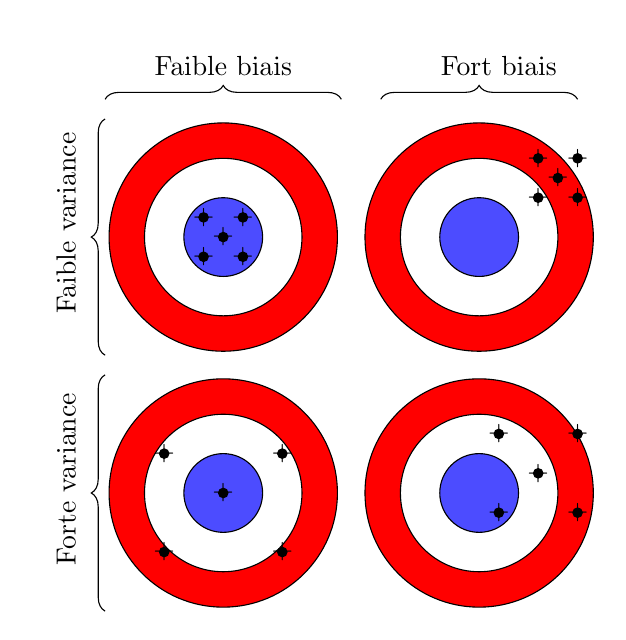
\begin{tikzpicture}
        \tikzset{
            brace/.style={decorate, decoration={brace, amplitude=5pt}},
            mbrace/.style={decorate, decoration={brace, amplitude=5pt, mirror}} 
        }
            \foreach \r/\col in {1.45cm/red, 1cm/white, .5cm/blue!70}{%
            \path[draw, fill=\col] (0,0) circle (\r) ;}
            %---%
            \foreach \coords in {(-.25,-.25),(.25,-.25), (0,0), (.25,.25),(-.25,.25)}{%
            \draw[fill=black] \coords circle (.6mm) node[]{+};}
            %---%
            \draw [brace] (-1.5,1.75) -- (1.5,1.75) ;
            \node[label, above=.5em] at(0,1.75) {Faible biais};
        \pause
            \foreach \r/\col in {1.45cm/red, 1cm/white, .5cm/blue!70}{%
            \path[draw,fill=\col] (3.25,0) circle (\r) ;}
            %---%
            \foreach \coords in {(4,.5), (4.5,.5), (4.25,.75), (4,1),(4.5,1)}{\draw[fill=black] \coords circle (.6mm) node[]{+};}
            %---%
            \draw [brace] (2, 1.75) -- (4.5, 1.75) ;
            \node[label, above=.5em] at(3.5, 1.75) {Fort biais};
        \pause
            \draw [brace] (-1.5, -1.5) -- (-1.5, 1.5) ;
            \node[label, above=.5em, rotate=90] at(-1.75, 0) {Faible variance};
        \pause
            \draw [mbrace] (-1.5, -1.75) -- (-1.5, -4.75) ;
            \node[label, above=.5em, rotate=90] at(-1.75, -3.25) {Forte variance};

            \foreach \r/\col in {1.45cm/red, 1cm/white, .5cm/blue!70}{%
            \path[draw,fill=\col] (0,-3.25) circle (\r) ;}
        
            \foreach \coords in {(-.75,-2.75), (.75,-2.75), (0,-3.25), (-.75,-4), (.75,-4)}{%
            \draw[fill=black] \coords circle (.6mm) node[]{+};}
        \pause
            \foreach \r/\col in {1.45cm/red, 1cm/white, .5cm/blue!70}{%
            \path[draw,fill=\col] (3.25,-3.25) circle (\r) ;}
        
            \foreach \coords in {(4,-3), (4.5,-2.5), (4.5,-3.5), (3.5,-2.5), (3.5,-3.5)}{%
            \draw[fill=black] \coords circle (.6mm) node[]{+};}
            %___%
        \end{tikzpicture}
    \end{column}
    \begin{column}{0.4\textwidth}
    \only<6->{
        Des estimateurs sans biais : \paut
        \pause
        \begin{itemize}
            \item moyenne :
            $ \hat{\mu} = \frac{1}{n}\sum_1^n x_i$
        \pause
            \item proportion :
            $ \hat{p} = \frac{\#succes}{n}$
        \pause
            \item variance (corrigée) :
            $$\displaystyle \hat{\sigma}^2 = \frac{\sum_1^n (x_i-\hat{\mu})^2}{n-1}$$ \paut
        \end{itemize}
        \pause
        Un estimateur biaisé
        \begin{itemize}
            \item variance :
            $$ \hat{s}^2 = \frac{\sum_1^n (x_i-\hat{\mu})^2}{n}$$
        \end{itemize}
    }
    \end{column}
    \end{columns}
\end{frame}
%---------------------------------%


%---------------------------------%
\begin{frame}[fragile]{Données binaires : estimer une proportion}
    Pour un échantillon de $n$ données, de valeurs 0 (échec) ou 1 (succès) : \pause
    \begin{itemize}
        \item un estimateur de la proportion de succes est : $\hat{p} = \frac{\#succes}{n}  \in \lbrack 0, 1\rbrack$, \pause
        \item la variance (de l'estimateur) est : $\hat{\sigma}^2=\frac{p\times(1-p)}{n}$,
        \only<8->{
        \item un IC$^*$ à $95\%$ pour $\hat{p}$ est : $\left [\hat{p} \pm 1.96\times\hat{\sigma} \right]$.
        }
    \end{itemize}
    \pause
    \begin{tikzpicture} \Huge
    \tikzset{matstyle/.style={matrix of nodes, nodes={rectangle, draw, white, minimum height=.25cm}},
        r/.style={fill=red!20},
        b/.style={fill=blue!20},}
        \matrix (m) [matstyle]{
        |[r]|&|[r]|&|[r]|&|[r]| & |[b]|&|[b]|&|[b]|&|[b]|\\
        |[r]|&|[r]|&|[r]|&|[r]| & |[b]|&|[b]|&|[b]|&|[b]|\\
        |[r]|&|[r]|&|[r]|&|[r]| & |[b]|&|[b]|&|[b]|&|[b]|\\
        |[r]|&|[r]|&|[r]|&|[r]| & |[b]|&|[b]|&|[b]|&|[b]|\\
        |[r]|&|[r]|&|[r]|&|[r]| & |[b]|&|[b]|&|[b]|&|[b]|\\
        |[r]|&|[r]|&|[r]|&|[r]| & |[b]|&|[b]|&|[b]|&|[b]|\\
        |[r]|&|[r]|&|[r]|&|[r]| & |[b]|&|[b]|&|[b]|&|[b]|\\
        |[r]|&|[r]|&|[r]|&|[r]| & |[b]|&|[b]|&|[b]|&|[b]|\\
        };
    \pause
        \draw[color=green!50!black, very thick] (m-5-4.north west) -- (m-5-5.north east) -- (m-6-5.south east) -- (m-6-4.south west) -- (m-5-4.north west);
    \only<4-6>{
        \node[color=green!50!black] (s) at (m-5-5.center){\tiny n=4};
        \node[color=green!50!black] (s) at (5,1.5){\small$\hat{p}=\frac{1}{2}$, $\hat{\sigma} = \sqrt{\frac{0.5\times(1-0.5)}{4}} = 0.25$.};
    }
    \only<5->{
        \draw[color=blue, very thick] (m-2-2.north west) -- (m-2-7.north east) -- (m-7-7.south east) -- (m-7-2.south west) -- (m-2-2.north west) ;
    }
    \only<5-6>{
        \node[color=blue] (s) at (m-7-7.west){\tiny n=36};
        \node[blue] (s) at (5,0){\small$\hat{p}=\frac{1}{2}$, $\hat{\sigma} = \sqrt{\frac{0.5\times(1-0.5)}{36}} \approx 0,08$.};
    }
    \only<6->{
        \draw[color=brown, very thick] (m-3-4.north west) -- (m-3-6.north east) -- (m-3-6.south east) -- (m-3-4.south west) -- (m-3-4.north west) ;
    }
    \only<6-6>{
        \node[color=brown] (s) at (m-3-6.center){\tiny n=3};
        \node[brown] (s) at (5,-1.5){\small$\hat{p}=\frac{1}{3}$, $\hat{\sigma} = \sqrt{\frac{0.33\times(1-0.33)}{3}} \approx 0,27$.};
    }
    \only<7->{
        \node[color=green!50!black] (s) at (m-5-5.west){\tiny n=40};
        \node[color=blue] (s) at (m-7-7.west){\tiny n=360};
        \node[color=brown] (s) at (m-3-6.west){\tiny n=30};
    }
    \only<7-7>{
        \node[color=green!50!black] (s) at (4.35, 1.5){\small$\hat{p}=\frac{1}{2}$, $\hat{\sigma} \approx 0,079$.};
        \node[blue] (s) at (4.35, 0){\small$\hat{p}=\frac{1}{2}$, $\hat{\sigma} \approx 0,026$.};
        \node[brown] (s) at (4.35, -1.5){\small$\hat{p}=\frac{1}{3}$, $\hat{\sigma} \approx 0,086$.};
    }
    \only<8->{
        \node[color=green!50!black] (s) at (6, 1.5){\small$\hat{p}=\frac{1}{2}$, $\hat{\sigma} \approx 0,079$, $IC_{95}(\hat{p})=[0.35; 0.65]$.};
        %%%
        \node[blue] (s) at (6, 0){\small$\hat{p}=\frac{1}{2}$, $\hat{\sigma} \approx 0,026$, $IC_{95}(\hat{p})= [0.45; 0.55]$.};
        %%%
        \node[brown] (s) at (6, -1.5){\small$\hat{p}=\frac{1}{3}$, $\hat{\sigma} \approx 0,086$, $IC_{95}(\hat{p})= [0.16; 0.50]$.};
    }
    \end{tikzpicture} \\
    \only<8->{$^* n\geq30, n\hat{p}\geq5, n(1-\hat{p})\geq5$.}
\end{frame}
%---------------------------------%



%--------------------------------------------------%
%--------------------------------------------------%
\section{Test statistique : comparaison de deux proportions}
%--------------------------------------------------%
%--------------------------------------------------%


%---------------------------------%
\begin{frame}{Test d'hypothèse : comparer une propotion à une référence}
    \underline{Contexte} : comparer une \tcb{proportion estimée $\hat{p}$} sur un $n$-échantillon, avec une \tco{proportion de référence $p_0$}. \paut \pause
    
    \underline{Exemple} : Depuis la réforme du lycée, la \tcb{part de filles}, parmis les élèves de maths, est elle significativement différente de \tco{la parité, $p_0\!=\!50\%$} ? \paut  \pause

    \underline{Hypothèses} : ${\cal H}_0 : \tco{p_0}=\tcb{\hat{p}}\quad$ contre $\quad{\cal H}_1 : \tco{p_0} \neq \tcb{\hat{p}}$. \paut  \pause

    \underline{Statistique de test} : $\hat{z} = \frac{\tco{p_0} - \tcb{\hat{p}}}{\sqrt{\frac{\tcb{\hat{p}}(1-\tcb{\hat{p}})}{n}}}\sim {\cal N}(0,1)$ sous l'hypothèse ${\cal H}_0$. \pause
    
    \underline{Conclusion} : au risque $\alpha\in[0,1]$, $\exists ! t_\alpha > 0 $  tq $P(-t_\alpha \leq \hat{z} \leq t_\alpha)=1-\alpha$. \\
    On rejette ${\cal H}_0$  si $\hat{z} < -t_{\alpha}$ ou $\hat{z} > t_{\alpha}$. %\paut

    \begin{center}
    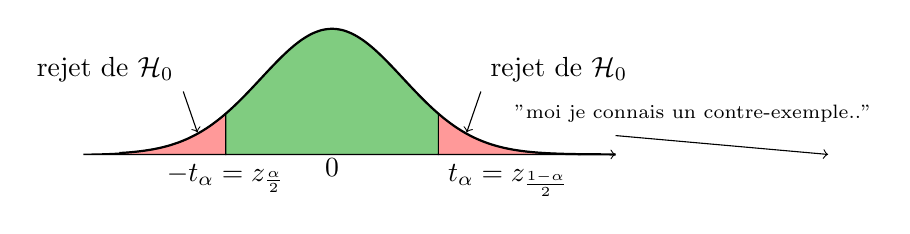
\begin{tikzpicture}[domain=-3:4,yscale=4, xscale=.9]
        \draw[->] (-3.5,0) -- (4,0);
        \filldraw[fill=red!40] (-3.5,0) -- plot[domain=-3.5:-1.5,smooth] (\x,{0.399*exp(-((\x)^2)/2)}) -- (-1.5,0) node[below]{$-t_{\alpha}=z_{\frac{\alpha}{2}}$} -- cycle ;
        \draw[<-] (-1.9, 0.07)--(-2.1, 0.2) node[above left]{rejet de ${\cal H}_0$} ;

        \filldraw[fill=red!40] (1.5,0) node[below right]{$t_{\alpha}=z_{\frac{1-\alpha}{2}}$} -- plot[domain=1.5:3.5,smooth] (\x,{0.399*exp(-((\x)^2)/2)}) -- (3.5,0) -- cycle;

        \filldraw[fill=green!60!black!50] (-1.5,0) -- plot[domain=-1.5:1.5,smooth] (\x,{0.399*exp(-((\x)^2)/2)}) -- (1.5,0) -- cycle;
        \draw[<-] (1.9, 0.07)--(2.1,0.2) node[above right]{rejet de ${\cal H}_0$} ;
        \draw[color=black,smooth,thick,samples=50] plot (\x,{0.399*exp(-((\x)^2)/2)});
        \node[above] at(0, -.1) {0};
        \pause
        \draw[->] (4,0.06)--(7, 0) node[above] at(5.1, .07) {\scriptsize \tcr{"moi je connais un contre-exemple.."}};
    \end{tikzpicture}
    \end{center}
\end{frame}
%---------------------------------%


%---------------------------------%
\begin{frame}{Exemples (1) : part des filles en maths au lycée}
    Sur les $149 540$ élèves qui ont choisi les mathématiques comme spécialité au baccalauréat 2021, $62 390$ sont des filles. [source] \paut \pause

    \underline{Proportion} : estimation de la part de filles parmis les élèves de maths :
    $$ \hat{p} = \frac{62 390}{149 540} \approx 0,417 
    \text{ avec } 
    IC_{95}(\hat{p})\approx [0.414; 0.419] .$$ \pause

    \underline{Statistique de test} : $\hat{z} = \frac{\tco{p_0} - \tcb{\hat{p}}}{\sqrt{\frac{\tcb{\hat{p}}(1-\tcb{\hat{p}})}{n}}} \approx 65$. \pause

    \underline{Conclusion} : au risque $\alpha = 5\%$, on a $t_\alpha=1.96$, et ici \textbf{\tcr{on rejette}} ${\cal H}_0$. \paut \pause

    \begin{center}
    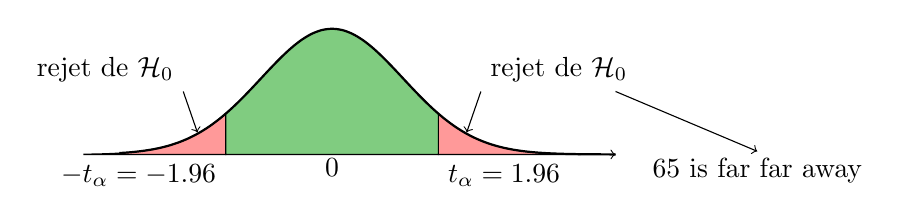
\begin{tikzpicture}[domain=-3:4,yscale=4, xscale=.9]
        \draw[->] (-3.5,0) -- (4,0);
        \filldraw[fill=red!40] (-3.5,0) -- plot[domain=-3.5:-1.5,smooth] (\x,{0.399*exp(-((\x)^2)/2)}) -- (-1.5,0) node[below left]{$-t_{\alpha}=-1.96$} -- cycle ;
        \draw[<-] (-1.9, 0.07)--(-2.1, 0.2) node[above left]{rejet de ${\cal H}_0$} ;

        \filldraw[fill=red!40] (1.5,0) node[below right]{$t_{\alpha}=1.96$} -- plot[domain=1.5:3.5,smooth] (\x,{0.399*exp(-((\x)^2)/2)}) -- (3.5,0) -- cycle;
        \node[above] at(0, -.1) {0};

        \filldraw[fill=green!60!black!50] (-1.5,0) -- plot[domain=-1.5:1.5,smooth] (\x,{0.399*exp(-((\x)^2)/2)}) -- (1.5,0) -- cycle;
        \draw[<-] (1.9, 0.07)--(2.1,0.2) node[above right]{rejet de ${\cal H}_0$} ;
        \draw[color=black,smooth,thick,samples=50] plot (\x,{0.399*exp(-((\x)^2)/2)});

        \pause
        \draw[<-] (6, 0.01)--(4,0.2) node[above] at(6, -.12) {\tcr{65 is far far away}};
    \end{tikzpicture}
    \end{center}
\end{frame}
%---------------------------------%


%---------------------------------%
\begin{frame}{Exemples (2) : part des femmes (MCF) en section 26}
    Sur les $1147$ MCF en section 26, $387$ sont des femmes. [source] \paut

    \underline{Proportion} : estimation de la part des femmes :
    $$ \hat{p} = \frac{387}{1147} \approx 0,34
    \text{ avec } 
    IC_{95}(\hat{p})\approx [0.31; 0.37] .$$

    \underline{Statistique de test} : $\hat{z} = \frac{\tco{p_0} - \tcb{\hat{p}}}{\sqrt{\frac{\tcb{\hat{p}}(1-\tcb{\hat{p}})}{n}}} \approx 11.$ \pause

    \underline{Conclusion} : au risque $\alpha = 5\%$, on a $t_\alpha=1.96$, et ici \textbf{\tcr{on rejette}} ${\cal H}_0$. \paut \pause

    \begin{center}
    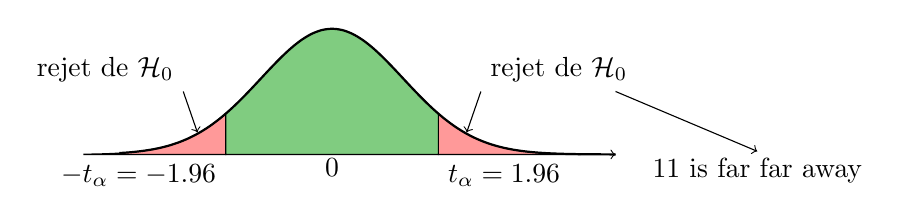
\begin{tikzpicture}[domain=-3:4,yscale=4, xscale=.9]
        \draw[->] (-3.5,0) -- (4,0);
        \filldraw[fill=red!40] (-3.5,0) -- plot[domain=-3.5:-1.5,smooth] (\x,{0.399*exp(-((\x)^2)/2)}) -- (-1.5,0) node[below left]{$-t_{\alpha}=-1.96$} -- cycle ;
        \draw[<-] (-1.9, 0.07)--(-2.1, 0.2) node[above left]{rejet de ${\cal H}_0$} ;

        \filldraw[fill=red!40] (1.5,0) node[below right]{$t_{\alpha}=1.96$} -- plot[domain=1.5:3.5,smooth] (\x,{0.399*exp(-((\x)^2)/2)}) -- (3.5,0) -- cycle;
        \node[above] at(0, -.1) {0};

        \filldraw[fill=green!60!black!50] (-1.5,0) -- plot[domain=-1.5:1.5,smooth] (\x,{0.399*exp(-((\x)^2)/2)}) -- (1.5,0) -- cycle;
        \draw[<-] (1.9, 0.07)--(2.1,0.2) node[above right]{rejet de ${\cal H}_0$} ;
        \draw[color=black,smooth,thick,samples=50] plot (\x,{0.399*exp(-((\x)^2)/2)});
        %\pause
        \draw[<-] (6, 0.01)--(4,0.2) node[above] at(6, -.12) {\tcr{11 is far far away}};
    \end{tikzpicture}
    \end{center}
    \pause
    Si $n\!=\!1147$, il faudrait $541$ femmes, soit $\hat{p}\!=\!0.471$ pour ne pas rejeter ${\cal H}_0$.
\end{frame}
%---------------------------------%


%---------------------------------%
\begin{frame}{Exemples (3) : part des femmes (PR) en section 26}
    Sur les $629$ MCF en section 25, $101$ sont des femmes. [source] \paut

    \underline{Proportion} : estimation de la part des femmes :
    $$ \hat{p} = \frac{101}{629} \approx 0,16
    \text{ avec } 
    IC_{95}(\hat{p})\approx [0.13; 0.19] .$$ %\pause

    \underline{Statistique de test} : $\hat{z} = \frac{\tco{p_0} - \tcb{\hat{p}}}{\sqrt{\frac{\tcb{\hat{p}}(1-\tcb{\hat{p}})}{n}}} \approx 23$. \pause

    \underline{Conclusion} : au risque $\alpha = 5\%$, on a $t_\alpha=1.96$, et ici \textbf{\tcr{on rejette}} ${\cal H}_0$. \paut \pause

    \begin{center}
    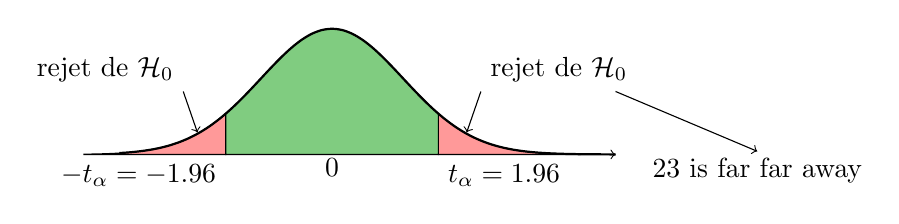
\begin{tikzpicture}[domain=-3:4,yscale=4, xscale=.9]
        \draw[->] (-3.5,0) -- (4,0);
        \filldraw[fill=red!40] (-3.5,0) -- plot[domain=-3.5:-1.5,smooth] (\x,{0.399*exp(-((\x)^2)/2)}) -- (-1.5,0) node[below left]{$-t_{\alpha}=-1.96$} -- cycle ;
        \draw[<-] (-1.9, 0.07)--(-2.1, 0.2) node[above left]{rejet de ${\cal H}_0$} ;

        \filldraw[fill=red!40] (1.5,0) node[below right]{$t_{\alpha}=1.96$} -- plot[domain=1.5:3.5,smooth] (\x,{0.399*exp(-((\x)^2)/2)}) -- (3.5,0) -- cycle;
        \node[above] at(0, -.1) {0};

        \filldraw[fill=green!60!black!50] (-1.5,0) -- plot[domain=-1.5:1.5,smooth] (\x,{0.399*exp(-((\x)^2)/2)}) -- (1.5,0) -- cycle;
        \draw[<-] (1.9, 0.07)--(2.1,0.2) node[above right]{rejet de ${\cal H}_0$} ;
        \draw[color=black,smooth,thick,samples=50] plot (\x,{0.399*exp(-((\x)^2)/2)});
        %\pause
        \draw[<-] (6, 0.01)--(4,0.2) node[above] at(6, -.12) {\tcr{23 is far far away}};
    \end{tikzpicture}
    \end{center}
    \pause
    Si $n\!=\!629$, il faudrait $290$ femmes, soit $\hat{p}=0.461$ pour ne pas rejeter ${\cal H}_0$.
\end{frame}
%---------------------------------%


%---------------------------------%
\begin{frame}{Exemples (4) : part des femmes (MCF) en section 25}
    Sur les $823$ MCF en section 25, $155$ sont des femmes. [source] \paut

    \underline{Proportion} : estimation de la part des femmes :
    $$ \hat{p} = \frac{155}{823} \approx 0,188 
    \text{ avec } 
    IC_{95}(\hat{p})\approx [0.162; 0.215] .$$

    \underline{Statistique de test} : $\hat{z} = \frac{\tco{p_0} - \tcb{\hat{p}}}{\sqrt{\frac{\tcb{\hat{p}}(1-\tcb{\hat{p}})}{n}}} \approx 23$. \pause

    \underline{Conclusion} : au risque $\alpha = 5\%$, on a $t_\alpha=1.96$, et ici \textbf{\tcr{on rejette}} ${\cal H}_0$. \paut \pause

    \begin{center}
    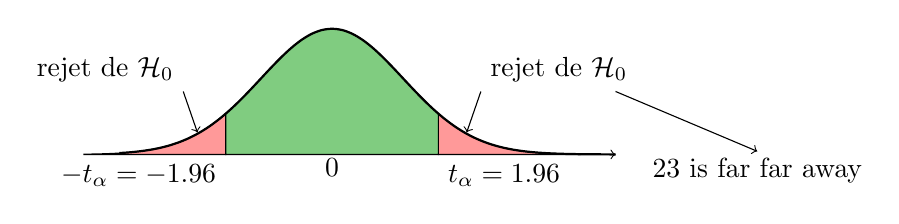
\begin{tikzpicture}[domain=-3:4,yscale=4, xscale=.9]
        \draw[->] (-3.5,0) -- (4,0);
        \filldraw[fill=red!40] (-3.5,0) -- plot[domain=-3.5:-1.5,smooth] (\x,{0.399*exp(-((\x)^2)/2)}) -- (-1.5,0) node[below left]{$-t_{\alpha}=-1.96$} -- cycle ;
        \draw[<-] (-1.9, 0.07)--(-2.1, 0.2) node[above left]{rejet de ${\cal H}_0$} ;

        \filldraw[fill=red!40] (1.5,0) node[below right]{$t_{\alpha}=1.96$} -- plot[domain=1.5:3.5,smooth] (\x,{0.399*exp(-((\x)^2)/2)}) -- (3.5,0) -- cycle;
        \node[above] at(0, -.1) {0};

        \filldraw[fill=green!60!black!50] (-1.5,0) -- plot[domain=-1.5:1.5,smooth] (\x,{0.399*exp(-((\x)^2)/2)}) -- (1.5,0) -- cycle;
        \draw[<-] (1.9, 0.07)--(2.1,0.2) node[above right]{rejet de ${\cal H}_0$} ;
        \draw[color=black,smooth,thick,samples=50] plot (\x,{0.399*exp(-((\x)^2)/2)});
        %\pause
        \draw[<-] (6, 0.01)--(4,0.2) node[above] at(6, -.12) {\tcr{23 is far far away}};
    \end{tikzpicture}
    \end{center}
    \pause
    Si $n\!=\!823$, il faudrait $383$ femmes, soit $\hat{p}=0.466$ pour ne pas rejeter ${\cal H}_0$.
\end{frame}
%---------------------------------%


%---------------------------------%
\begin{frame}{Exemples (5) : part des femmes (PR) en section 25}
    Sur les $498$ PR en section 25, $31$ sont des femmes. [source] \paut

    \underline{Proportion} : estimation de la part des femmes :
    $$ \hat{p} = \frac{31}{498} \approx 0,06 
    \text{ avec } 
    IC_{95}(\hat{p})\approx [0.04; 0.08] .$$ %\pause

    \underline{Statistique de test} : $\hat{z} = \frac{\tco{p_0} - \tcb{\hat{p}}}{\sqrt{\frac{\tcb{\hat{p}}(1-\tcb{\hat{p}})}{n}}} \approx 40$. \pause

    \underline{Conclusion} : au risque $\alpha = 5\%$, on a $t_\alpha=1.96$, et ici \textbf{\tcr{on rejette}} ${\cal H}_0$. \paut \pause

    \begin{center}
    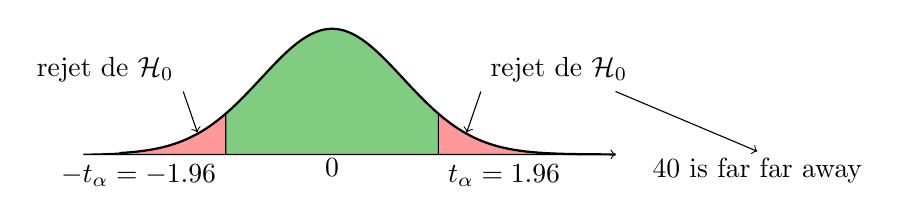
\begin{tikzpicture}[domain=-3:4,yscale=4, xscale=.9]
        \draw[->] (-3.5,0) -- (4,0);
        \filldraw[fill=red!40] (-3.5,0) -- plot[domain=-3.5:-1.5,smooth] (\x,{0.399*exp(-((\x)^2)/2)}) -- (-1.5,0) node[below left]{$-t_{\alpha}=-1.96$} -- cycle ;
        \draw[<-] (-1.9, 0.07)--(-2.1, 0.2) node[above left]{rejet de ${\cal H}_0$} ;

        \filldraw[fill=red!40] (1.5,0) node[below right]{$t_{\alpha}=1.96$} -- plot[domain=1.5:3.5,smooth] (\x,{0.399*exp(-((\x)^2)/2)}) -- (3.5,0) -- cycle;
        \node[above] at(0, -.1) {0};

        \filldraw[fill=green!60!black!50] (-1.5,0) -- plot[domain=-1.5:1.5,smooth] (\x,{0.399*exp(-((\x)^2)/2)}) -- (1.5,0) -- cycle;
        \draw[<-] (1.9, 0.07)--(2.1,0.2) node[above right]{rejet de ${\cal H}_0$} ;
        \draw[color=black,smooth,thick,samples=50] plot (\x,{0.399*exp(-((\x)^2)/2)});

        %\pause
        \draw[<-] (6, 0.01)--(4,0.2) node[above] at(6, -.12) {\tcr{40 is far far away}};
    \end{tikzpicture}
    \end{center}
    \pause
    Si $n\!=\!498$, il faudrait $228$ femmes, soit $\hat{p}=0.457$ pour ne pas rejeter ${\cal H}_0$.
\end{frame}
%---------------------------------%


%--------------------------------------------------%
%--------------------------------------------------%
\section{Test d'indépendance : de deux caractéristiques}
%--------------------------------------------------%
%--------------------------------------------------%


%---------------------------------%
\begin{frame}{Test d'indépendance de deux variables}
    \underline{Contexte} : comparer des \tcb{effectifs observés} de deux caractéristiques $X$ et $Y$, avec des \tco{effectifs théoriques issus de variables indépendantes}. \paut \pause
    
    \underline{Exemple} : On note $X$ la v.a \textit{genre} et $Y$ la v.a \textit{faire des maths au lycée}. 
    \begin{columns}
        \begin{column}{0.4\textwidth} \scriptsize
        {\renewcommand{\arraystretch}{1.1}\tabcolsep2pt
		\begin{tabular}{|c|c|c|c|} 
			\hline
			$O_{ij}$     &  F      &  G      & total   \\ \hline
			maths        & \tcb{62 390} & \tcb{87 150} & 149 540 \\ \hline
			\sout{maths} & \tcb{147 663} & \tcb{74 502} & 222 165 \\ \hline
            total        & 210 053 & 161 652 & 371 705 \\ \hline
		\end{tabular}}
        \end{column}
        \pause
        \begin{column}{0.17\textwidth} \scriptsize
            $ T_{ij} \!=\! \frac{(O_{i+} \times O_{+j})}{n}$ \\
            $ O_{i+} \!=\! \sum_j O_{ij} $ \\
            $ O_{+j} \!=\! \sum_i O_{ij} $ \\
        \end{column}
        \pause
        \begin{column}{0.41\textwidth} \scriptsize
        {\renewcommand{\arraystretch}{1.1}\tabcolsep2pt
        \begin{tabular}{|c|c|c|c|}
            \hline
            $ T_{ij} $   &  F      &     G   & total \\ \hline
            maths        & \tco{84 506}  & \tco{65 034} & 149 540 \\ \hline
            \sout{maths} & \tco{125 547} & \tco{96 618} & 222 165 \\ \hline
            total        & 210 053 & 161 652 & 371 705 \\ \hline
        \end{tabular}}
        \end{column}
	\end{columns} \paut \pause

    \underline{Hypothèses} : {\small ${\cal H}_0 : X \ind Y $ vs $ {\cal H}_1$ : $X \nind Y$, $\hat{z} = \sum_{i,j} \frac{(O_{i,j}-T_{i,j})^2}{T_{i,j}} \sim {\cal X}^2_1$ sous ${\cal H}_0$.} \paut \pause

    \underline{Conclusion} : au risque  $\alpha \!\!=\!\! 5\%$, on rejette ${\cal H}_0$  si \tco{$\hat{z} \!\!>\!\! t_{\alpha}\!\!=\!\!3.84$}. 
    \pause
    Ici, \tcr{$\hat{z}\!=\!22266$}.

    \begin{center}
        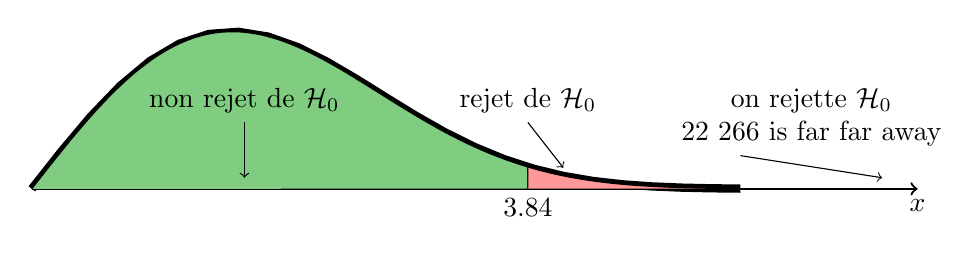
\begin{tikzpicture}[y=.08pt, x=9cm]
            % axis
            \draw [thick] [->] (0,0)--(1.25,0) node[right, below] {$x$};
            %\draw [thick] [->] (0,0)--(0,1000) node[above, left] {$y$};
            % curve
            \draw [domain=0:1, variable=\x, line width=3pt] plot (\x, {\x*(2-(\x)^2)^12}); %, samples=2000
            % not rejecting H0 area
            \filldraw[fill=green!60!black!50] (0,0) -- plot[domain=0:.7,smooth] (\x,{\x*(2-(\x)^2)^12}) -- (.7,.7);
            \draw[<-] (.3, 50)--(.3, 300) node at (.3, 400) {non rejet de ${\cal H}_0$} ;
            % rejecting H0 area
            \node[below] at (.7,.7) {3.84} ;
            \filldraw[fill=red!40] (.7,.7) -- plot[domain=.7:1,smooth] (\x,{\x*(2-(\x)^2)^12});
            \draw[<-] (.75, 95)--(.7, 300) node at (.7, 400) {rejet de ${\cal H}_0$} ;
            \pause
            \node at (1.1, 400) {\tcr{on rejette ${\cal H}_0$}} ;
            \draw[<-] (1.2, 50)--(1, 150) node at (1.1, 250) {\tcr{22 266 is far far away}} ;
        \end{tikzpicture}
    \end{center}
\end{frame}
%---------------------------------%


%--------------------------------------------------%
%--------------------------------------------------%
\section{Conclusions}
%--------------------------------------------------%
%--------------------------------------------------%


%---------------------------------%
\begin{frame}{Quelques ressources}
   \begin{center}
       \begin{itemize}
            \item chiffres filles et maths au lycée : \\
            \url[test]{https://femmes-et-maths.fr/2022/03/17/30-des-filles-et-54-des-garcons-ont-presente-la-specialite-maths-au-baccalaureat-2021/} \paut

            \item chiffres femmes et maths (MCF \& PR 25, 26) : \\
            \url{https://femmes-et-maths.fr/wp-content/uploads/2020/02/journéeParité4BROZE.pdf} \paut

            \item Pour un regard objectif/quantifié sur les stéréotypes : \\ 
            \url{https://femmes-et-maths.fr/wp-content/uploads/2021/03/Brochure_Grand_Public_interactif.pdf} \paut
       \end{itemize}
   \end{center}
\end{frame}
%---------------------------------%


%---------------------------------%
% \begin{frame}[fragile]{Formalisons}
%     \begin{block}{Loi de Bernouilli $\mathcal{B}(p)$, avec $p \in [0, 1]$}
%         On dit qu'une variable aléatoire $X$, suit une loi de Bernouilli si \\
%         $ \mathbb{P}(X=1) = p \text{ et } \mathbb{P}(X=0) = 1-p,$ \\
%         et on note $X \sim \mathcal{B}(p)$, où $p$ est inconnu et estimé par $\hat{P} = \frac{1}{n}\sum_1^n X_i$.
%     \end{block} %alert %example

%     \begin{block}{Application du TCL}
%         Si $X_i \!\sim\! \mathcal{B}(p)$, $i\!=\!\llbracket1,n\rrbracket$, $\hat{P}$ suit une loi Binomiale, et on note $\hat{P} \!\sim\! \mathcal{B}(n, p)$. \\
%         % Alors, lorsque $n$ est grand, $\frac{\hat{P}-p}{\sqrt{\frac{p(1-p)}{n}}}$ se rapproche de la loi $\mathcal{N}(0, 1)$. \\
%         % Une estimation par intervalle de $\hat{P}$ est $\left [\hat{P} \pm 1.96\sqrt{\frac{\hat{P}(1-\hat{P})}{n}} \right]$. 
%         Si $n$ est grand, un IC$_{95\%}$ de $\hat{P}$ est $\left [\hat{P} \pm 1.96\sqrt{\frac{\hat{P}(1-\hat{P})}{n}} \right]$, et $z=\frac{\hat{P}-p}{\sqrt{\frac{p(1-p)}{n}}}$ se rapproche de la loi $\mathcal{N}(0, 1)$.
%     \end{block} % 

%     \begin{block}{Test de comparaison d'une proportion à une valeur de référence}
%         On teste l'hypothèse $\mathcal{H}_0 : \hat{P}=p$ vs l'alternative $\mathcal{H}_1 : \hat{P}\neq p$. \\
%         On rejette $\mathcal{H}_0$ (au profit de $\mathcal{H}_1$) si $z \notin$
%     \end{block}
% \end{frame}
%---------------------------------%


%---------------------------------%
% \begin{frame}
%     \begin{figure}[H]
%     \centering
%     \begin{tikzpicture}[declare function={binom(\k,\n,\p)=\n!/(\k!*(\n-\k)!)*\p^\k*(1-\p)^(\n-\k);}]
%         \begin{axis}[width=9cm,ymin=0, xmin=-0.5, xmax=17, axis lines=left,xlabel={\scriptsize\scriptsize$k$}, ylabel={\scriptsize$f(x)$}, x label style={at={(axis description cs:1,0)},anchor=west},
%         y label style={at={(axis description cs:0,1)},rotate = -90, anchor=south}, ,
%         samples at={0,...,16},
%         yticklabel style={font=\scriptsize,
%             /pgf/number format/fixed,
%             /pgf/number format/fixed zerofill,
%             /pgf/number format/precision=2},
%         ybar=0pt, bar width=1, bar shift=0pt, xticklabel style={font=\scriptsize},xticklabel style={font=\scriptsize}]
%         \addplot [fill=gray!25] {binom(x,20,0.4)}; 
%         \end{axis}
%         \end{tikzpicture}
%     \end{figure}
% \end{frame}
%---------------------------------%


%---------------------------------%
% \begin{frame}
% \begin{tikzpicture}
%     \begin{axis}
%     [% Define probability distribution functions
%         declare function={
%             binom(\n,\p) = \n!/(x!*(\n-x)!)*\p^x*(1-\p)^(\n-x);
%             normal(\m,\s) = 1/(\s*sqrt(2*pi))*exp(-((x-\m)^2)/(2*\s^2));
%         },
%         % Plotting options
%         title=Binomial \& Normal Distribution,
%         xlabel={$x$}, ylabel={$f(x)$},
%         ymin=0, ymax=.3,
%         samples at={0,...,30},
%         xtick style={draw=none},
%         yticklabel style={
%             /pgf/number format/fixed,
%             /pgf/number format/fixed zerofill,
%             /pgf/number format/precision=2,
%         },   
%     ]
    
%     % Plot Binomial Distribution
%     \addplot [ybar=0pt,bar width=1pt,fill=black] {binom(40,0.5)};  
%     \addlegendentry{$B(40,0.5)$}
    
%     % Plot Normal Distribution (1)
%     \addplot [smooth,red,thick] {normal(20,3)}; 
%     \addlegendentry{$\mathcal{N}(20,3^2)$}
%     \end{axis}
%     \end{tikzpicture}
% \end{frame}
%---------------------------------%


\end{document}

